\newpage
\section{Экспериментальная часть}

Проведем тестирование и сравним алгоритмы по времени работы.

\subsection{Примеры работ}

Ниже приведены примеры работ при корректных и некорректных данных

\begin{figure}[H]
    \centering
    
\includegraphics[scale=0.5]{zero_arg}
    \caption{Без аргументов}
    \label{img:zero-arg}
\end{figure}

\begin{figure}[H]
    \centering
    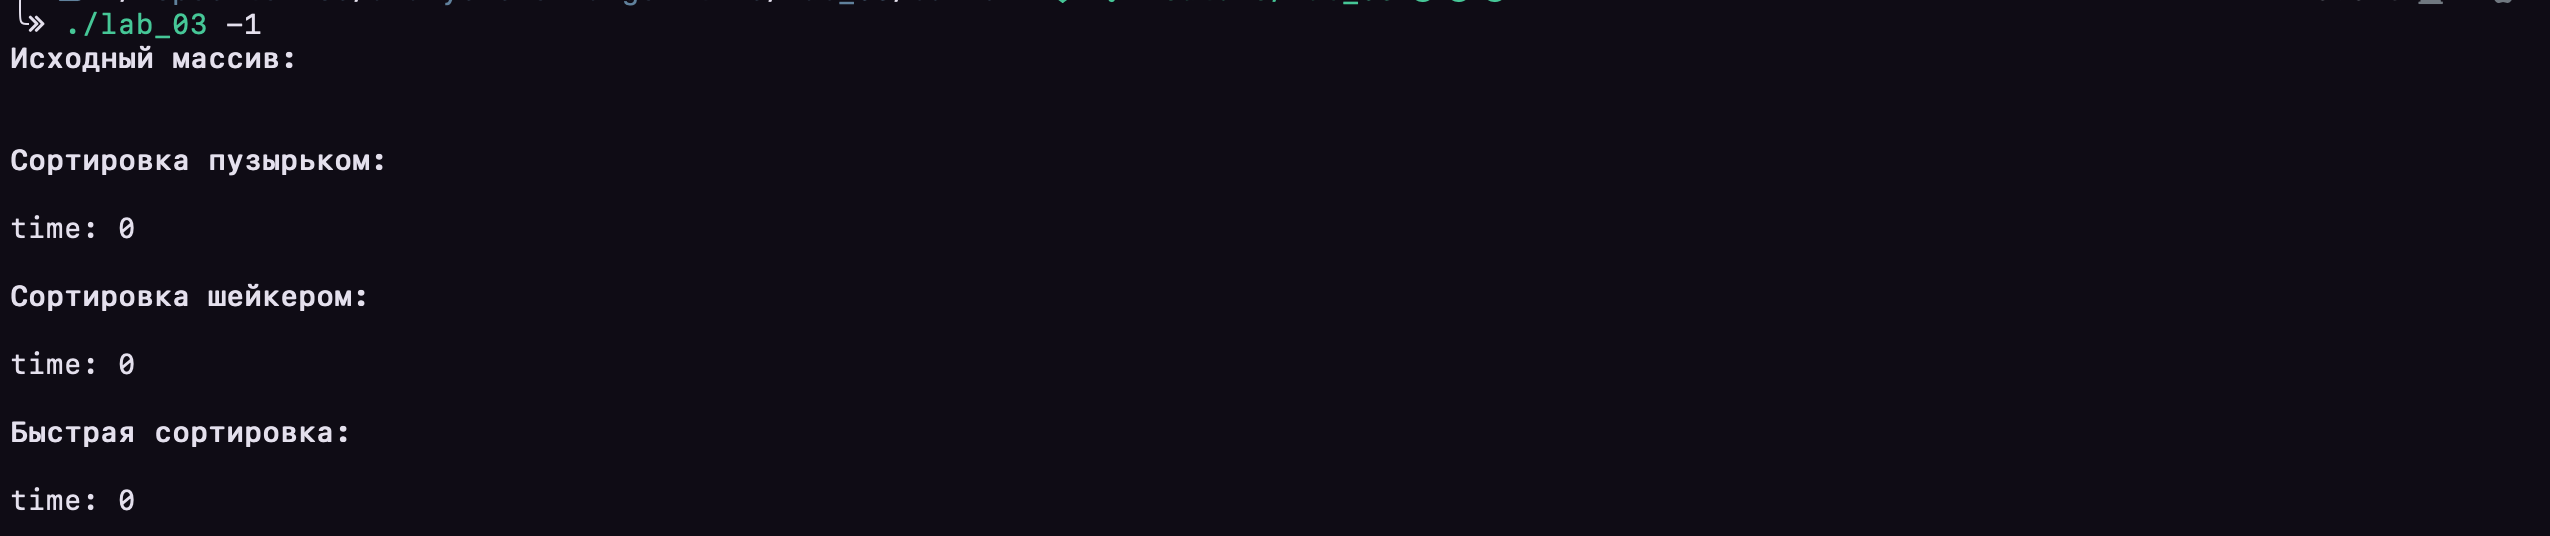
\includegraphics[scale=0.5]{less_zero}
    \caption{Некорректный аргумент}
    \label{img:less-arg}
\end{figure}

\begin{figure}[H]
    \centering
    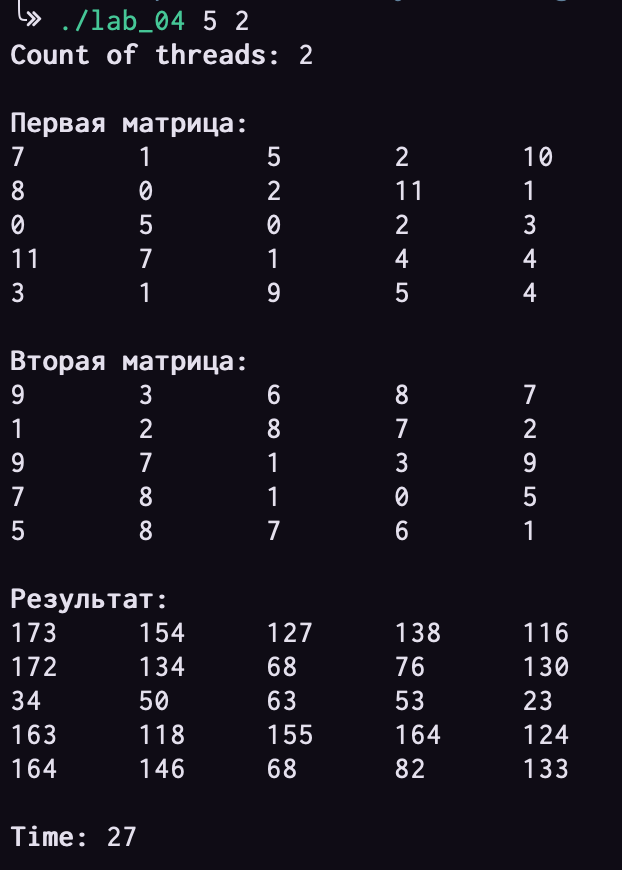
\includegraphics[scale=1]{five}
    \caption{Работа 2 потоков}
    \label{img:five}
\end{figure}

\begin{figure}[H]
    \centering
    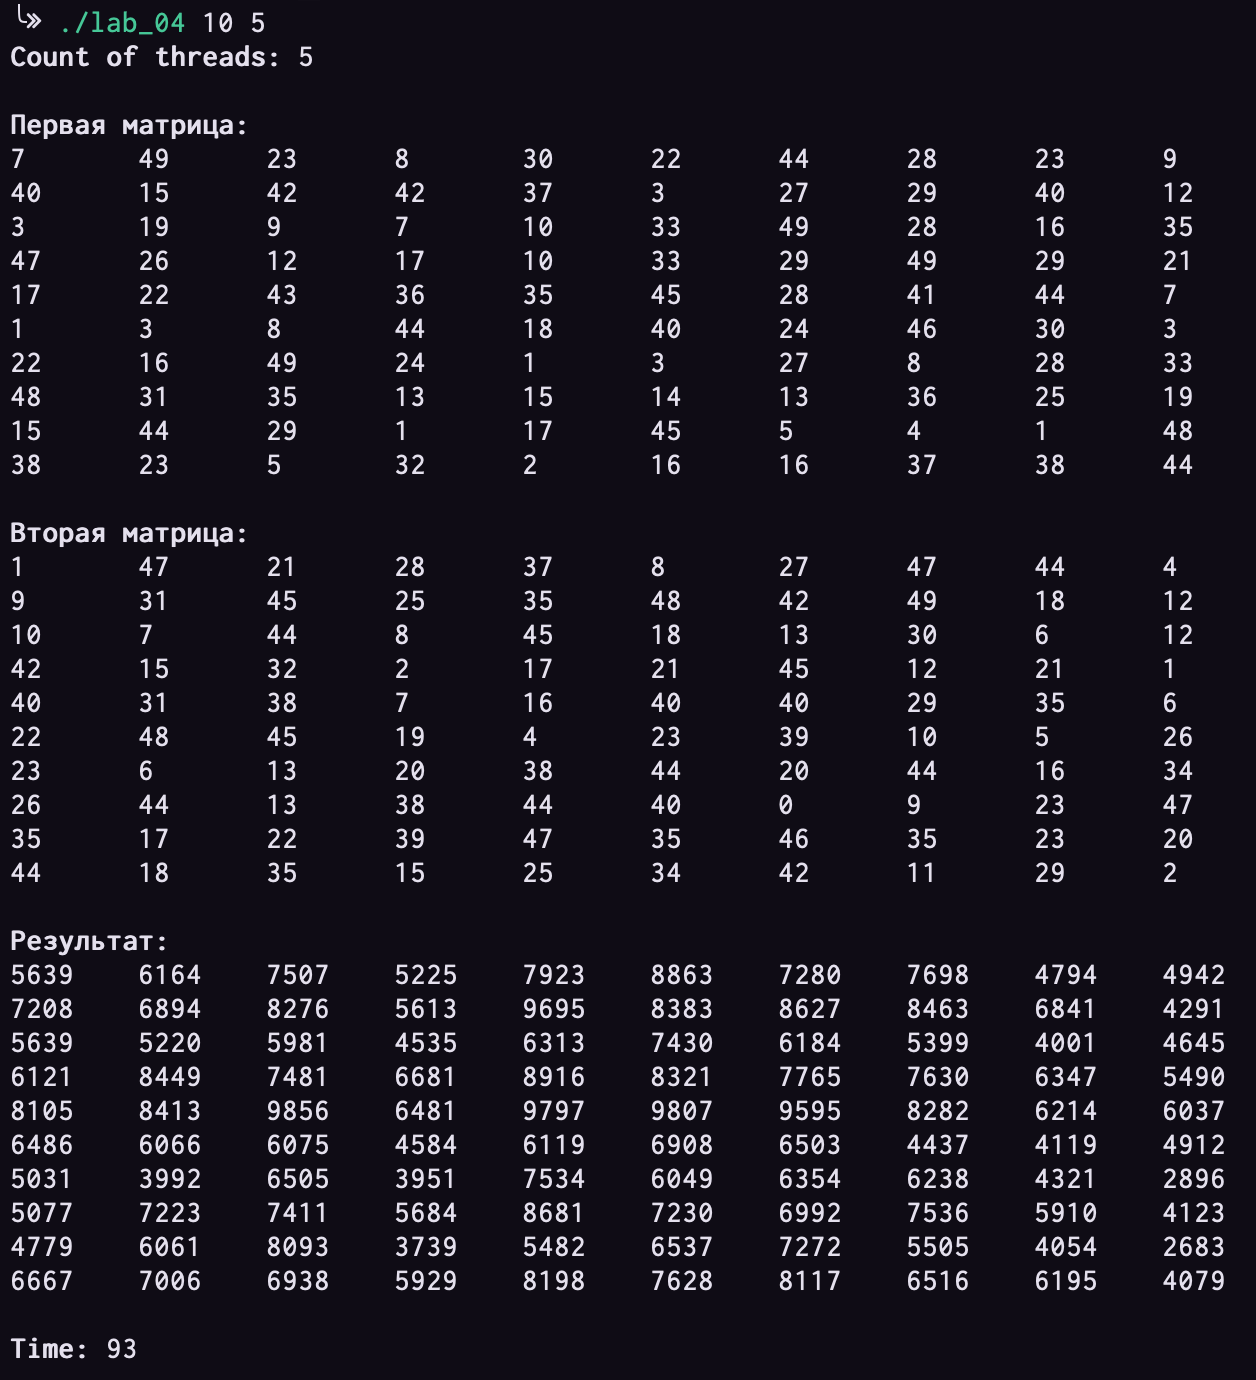
\includegraphics[scale=0.6]{ten}
    \caption{Работа 5 потоков}
    \label{img:ten}
\end{figure}

\subsection{Результаты тестирования}

Для тестирования были использованы тесты в таблице \ref{table:test}.
Результаты продемонстрированы в таблицах \ref{table:test-res} и \ref{table:test-res-th}.

\begin{table}[H]
    \caption{Результаты однопоточного алгоритма}
    \label{table:test-res}
    \centering
    \begin{tabular}{|c|c|c|}
        \hline
        Первая матрца & Вторая матрица & Результат \\
        \hline
        1 2 & 1 2 & \ 7 10 \\
        3 4 & 3 4 & 15 22 \\
        \hline
        1 2 3 & 1 2 3 & \ 30\ \ 36\ \ 42 \\
        4 5 6 & 4 5 6 & \ 66\ \ 81\ \ 96 \\
        7 8 9 & 7 8 9 & 102 126 150 \\
        \hline
        1 2 3 & 1 & 14 \\
        4 5 6 & 2 & 32 \\
              & 3 & \\
        \hline
    \end{tabular}
\end{table}

\begin{table}[H]
    \caption{Результаты многопоточного алгоритма}
    \label{table:test-res-th}
    \centering
    \begin{tabular}{|c|c|c|}
        \hline
        Первая матрца & Вторая матрица & Результат \\
        \hline
        1 2 & 1 2 & \ 7 10 \\
        3 4 & 3 4 & 15 22 \\
        \hline
        1 2 3 & 1 2 3 & \ 30\ \ 36\ \ 42 \\
        4 5 6 & 4 5 6 & \ 66\ \ 81\ \ 96 \\
        7 8 9 & 7 8 9 & 102 126 150 \\
        \hline
        1 2 3 & 1 & 14 \\
        4 5 6 & 2 & 32 \\
              & 3 & \\
        \hline
    \end{tabular}
\end{table}  

Все тесты пройдены успешно.

\subsection{Замеры времени}

На рисунке \ref{img:even} представлены результаты замера времени алгоритмов при
четных размерностях, а на рисунке \ref{img:noteven} при нечетных размерностях матриц.
Оба случая прогонялись на квардатных матрицах.

\begin{figure}[H]
    \begin{tikzpicture}
        \begin{axis}[
            legend pos = north west,
            xlabel=Размерность матрицы,
            ylabel=микросекунды,
            grid = major,
            width = 0.8\paperwidth,
            height = 0.38\paperheight,
            line width = 1
        ]
            \legend{
                1 поток,
                2 потока,
                4 потока,
                8 потоков,
                16 потоков
            };
            \addplot coordinates {
                (100, 14628)
                (200, 116180)
                (300, 438016)
                (400, 1187214)
                (500, 2385626)
                (600, 4243078)
                (700, 6698034)
                (800, 10465285)
                (900, 21069337)
                (1000, 27797876)
            };

            \addplot coordinates {
                (100, 8757)
                (200, 64567)
                (300, 220776)
                (400, 618716)
                (500, 1229652)
                (600, 2113989)
                (700, 3375514)
                (800, 5236305)
                (900, 11378200)
                (1000, 17093862)
            };

            \addplot coordinates {
                (100, 4715)
                (200, 60202)
                (300, 172877)
                (400, 553051)
                (500, 1066518)
                (600, 1929989)
                (700, 3044136)
                (800, 4601543)
                (900, 8663647)
                (1000, 14690104)
            };

            \addplot coordinates {
                (100, 7619)
                (200, 45675)
                (300, 174078)
                (400, 469850)
                (500, 1036757)
                (600, 1803543)
                (700, 2952666)
                (800, 4592266)
                (900, 7127271)
                (1000, 13610609)
            };

            \addplot coordinates {
                (100, 9139)
                (200, 32580)
                (300, 151308)
                (400, 433387)
                (500, 944650)
                (600, 1666263)
                (700, 3051969)
                (800, 4548904)
                (900, 8071541)
                (1000, 12539912)
            };
        \end{axis}
    \end{tikzpicture}
    \caption{Четная размерность}
    \label{img:even}
\end{figure}

\begin{figure}[H]
    \begin{tikzpicture}
        \begin{axis}[
            legend pos = north west,
            xlabel=Размерность матрицы,
            ylabel=микросекунды,
            grid = major,
            width = 0.8\paperwidth,
            height = 0.38\paperheight,
            line width = 1
        ]
            \legend{
                1 поток,
                2 потока,
                4 потока,
                8 потоков,
                16 потоков
            };

            \addplot coordinates {
                (101, 15213)
                (201, 117837)
                (301, 443410)
                (401, 1220647)
                (501, 2392950)
                (601, 4218498)
                (701, 6738488)
                (801, 10540792)
                (901, 18951786)
                (1001, 28697609)
            };

            \addplot coordinates {
                (101, 8774)
                (201, 59229)
                (301, 224074)
                (401, 628244)
                (501, 1219904)
                (601, 2159161)
                (701, 3455919)
                (801, 5280501)
                (901, 10318001)
                (1001, 16102750)
            };

            \addplot coordinates {
                (101, 9212)
                (201, 58437)
                (301, 207268)
                (401, 538472)
                (501, 1048101)
                (601, 1907731)
                (701, 2988553)
                (801, 4593652)
                (901, 8808202)
                (1001, 14225764)
            };

            \addplot coordinates {
                (101, 8624)
                (201, 41359)
                (301, 129048)
                (401, 464942)
                (501, 1025854)
                (601, 1799975)
                (701, 2930749)
                (801, 4621777)
                (901, 8195691)
                (1001, 12314462)
            };

            \addplot coordinates {
                (101, 9228)
                (201, 33492)
                (301, 138411)
                (401, 425481)
                (501, 934565)
                (601, 1746171)
                (701, 3141964)
                (801, 4555403)
                (901, 8106159)
                (1001, 14064880)
            };
        \end{axis}
    \end{tikzpicture}
    \caption{Нечетная размерность}
    \label{img:noteven}
\end{figure}

\subsection{Выводы}

Из графиков отношения размерности матрицы ко времени вычисления видно, что рассчет
на одном потоке работает в 2 раза медленнее вычислений на нескольких потоках.
Среди распараллеленных вычислений видно, что увеличение числа потоков дает
небольшой прирост к скорости примерно на 5\%. Но чем больше потоков используется, тем
этот прирост меньше. На графике с четной размерностью можно заметить, что на 1000
размерности 16 потоков начинают проигрывать по скорости 8 потокам.
